%Dies ist die Hauptseite des Dokumentes. Es werden u. a. alle Kapitel,
%Einstellung im Header eingebunden.  Veränderungen müssen in folgenden Dateien
%vorgenommen werden:
      %- Layout.tex
      %- newComments.tex
      %- Titelseite
      %- Versionsübersicht
      %- einzelne Kapitel (evtl. erweitern)

% Definition von globalen Parametern, die derzeit auf der Titelseite und in der
% Kopfzeile verwendet werden. Der in <> gesetzte Text ist zu verändern.

\newcommand{\praktikumTitel}{WiReLib}
\newcommand{\projektTitel}{WiReLib}


%Hier sind alle Einstellungen enthalten, die sich auf das Seiten- und
%Dokumentenlayout beziehen

\documentclass[
  11pt,                % Schriftgröße
  DIV12,
  german,              % für Umlaute, Silbentrennung etc.
  oneside,            % einseitiges Dokument
  titlepage,          % es wird eine Titelseite verwendet
  parskip=half,        % Abstand zwischen Absätzen (halbe Zeile)
  headings=normal,      % Größe der Überschriften verkleinern
  captions=tableheading,  % Beschriftung von Tabellen unterhalb ausgeben
  final                % Status des Dokuments (final/draft)
]{scrreprt}            %


%------Ändern von Schriftschnitten - (Muss ganz am Anfang stehen !) ------------
\usepackage{fix-cm}

%------Umlaute -----------------------------------------------------------------
%   Umlaute/Sonderzeichen wie äüöß können direkt im Quelltext verwenden werden.
%    Erlaubt automatische Trennung von Worten mit Umlauten.
\usepackage[T1]{fontenc}
\usepackage[utf8]{inputenc}

%------Anpassung der Landessprache----------------------------------------------
\usepackage{ngerman}

%------Einfache Definition der Zeilenabstände und Seitenränder------------------
\usepackage{geometry}
\usepackage{setspace}
\usepackage{xspace}

%------Schriftgrößenanpassung von einzelnen Textpassagen------------------------
\usepackage{relsize}

%------Trennlinien in Kopf- und Fusszeile
\usepackage[headsepline, footsepline, ilines]{scrpage2}

%------Grafiken-----------------------------------------------------------------
\usepackage{graphicx}

%------Packet zum Sperren, Unterstreichen und Hervorheben von Texten------------
\usepackage{soul}

%------ergänzende Schriftart----------------------------------------------------
\usepackage{helvet}

%------Lange Tabellen-----------------------------------------------------------
\usepackage{longtable}
\usepackage{array}
\usepackage{ragged2e}
\usepackage{lscape}

%------PDF-Optionen-------------------------------------------------------------
\usepackage[
  bookmarks,
  bookmarksopen=true,
  colorlinks=true,
  linkcolor=black,        % einfache interne Verknüpfungen
  anchorcolor=black,      % Ankertext
  citecolor=black,        % Verweise auf Literaturverzeichniseinträge im Text
  filecolor=black,        % Verknüpfungen, die lokale Dateien öffnen
  menucolor=black,        % Acrobat-Menüpunkte
  urlcolor=black,         % Farbe für URL-Links
  backref,                % Zurücktext nach jedem Bibliografie-Eintrag als
                          % Liste von Überschriftsnummern
  pagebackref,            % Zurücktext nach jedem Bibliografie-Eintrag als
                          % Liste von Seitenzahlen
  plainpages=false,       % zur korrekten Erstellung der Bookmarks
  pdfpagelabels,          % zur korrekten Erstellung der Bookmarks
  hypertexnames=false,    % zur korrekten Erstellung der Bookmarks
  linktocpage             % Seitenzahlen anstatt Text im Inhaltsverzeichnis
                          % verlinken
  ]{hyperref}

%-----Glossar-Optionen----------------------------------------------------------
\usepackage{translator}
\usepackage[				   %
acronym,		% ein Abkürzungsverzeichnis erzeugen
toc,			% Taucht im Inhaltsverzeichnis auf
]				   
{glossaries}
\makeglossaries

\usepackage{xcolor}
\definecolor{lightergray}{rgb}{0.9,0.9,0.9}

\usepackage{listings}
\lstset{numbers=left, numberstyle=\tiny, numbersep=5pt,
breaklines=true, backgroundcolor=\color{lightergray},
basicstyle=\ttfamily,
}
\usepackage{booktabs}
      % enthält eingebundene Packete

%------Seitenränder-------------------------------------------------------------
\geometry{verbose,                     % zeigt die eingestellten Parameter beim
                                       % Latexlauf an
      paper=a4paper,                   % Papierformat
      top=25mm,                        % Rand oben
      left=25mm,                       % Rand links
      right=25mm,                      % Rand rechts
      bottom=45mm,                     % Rand unten
      pdftex                           % schreibt das Papierformat in die
                                       % Ausgabe damit Ausgabeprogramm
                                       % Papiergröße erkennt
  }

%Seitenlayout
\onehalfspace        % 1,5-facher Abstand

%------Kopf- und Fußzeilen -----------------------------------------------------
\pagestyle{scrheadings}

%------Kopf- und Fußzeile auch auf Kapitelanfangsseiten ------------------------
\renewcommand*{\chapterpagestyle}{scrheadings}

%------Schriftform der Kopfzeile -----------------------------------------------
\renewcommand{\headfont}{\normalfont}

%------Kopfzeile----------------------------------------------------------------
\setlength{\headheight}{21mm}        % Höhe der Kopfzeile
\ihead{\large{\textsc{\praktikumTitel}}\\    % Text in der linken Box
       \small{\projektTitel}}
\chead{}                            % Text in der mittleren Box

%----Fusszeile
\cfoot{}                            % Text in mittlerer Box
\ofoot{\pagemark}                    % Seitenzahl in rechter Box
          % Diese Datei enthält alle
                                          % Layouteinstellungen

% Dieses Befehle sortieren die Einträge in den einzelnen Listen:
%makeindex -s datei.ist -t datei.alg -o datei.acr datei.acn
%makeindex -s datei.ist -t datei.glg -o datei.gls datei.glo
%makeindex -s datei.ist -t datei.slg -o datei.syi datei.syg

% Kapitel 9
%-------------------------------------------------------------------------------
%Hier werden Fachbegriffe und Abkürzungen erklährt.
% Verwendet werden diese Begriffe mit \gls{name} oder \Gls{name} wenn der Anfang
% groß geschrieben sein muss.
%
%%	Beispiel unter: http://ewus.de/tipp-1029.html
%%	und natürlich Erkärung mit dem Befehl
%texdoc glossaries

\newacronym{UB}{UB}{Universitätsbibliothek}
\newacronym{GITZ}{GITZ}{Gauß-IT-Zentrum}
\newacronym{LDAP}{LDAP}{Lightweight Directory Access Protocol\protect\glsadd{glos:LDAP}}

% nur über \gls{LDAP} verwenden.
\newglossaryentry{glos:LDAP}{name=Lightweight Directory Access Protocol,
description={LDAP ist ein Verzeichnisdienst der von der TU Braunschweig für die Benutzerauthentifizierung bereit gestellt wird}
}
\newglossaryentry{glos:https}{name=Hypertext Transfer Protocol Secure,
description={Hypertext Transfer Protocol Secure ist die verschlüsselte Variante
vom Hypertext Transfer Protocol und ist eine zertifiktasbasierende sichere
Übertragungstechnik}
}
\newglossaryentry{glos:sqlite}{name=SQLite,
description={SQLite ist eine Relationale Datenbank die von Python direkt zur Verfügung gestellt wird}
}
\newglossaryentry{glos:copdes}{name=Corporate Design,
description={Das Corporate Design ist das gemeinsame Erscheinungsbild eine Unternehmens. Dies bezieht sich unter anderem auf Kommmunikationsmittel, Werbemittel und Internetauftritte}
}
\newglossaryentry{glos:unicode}{name=Unicode,
description={Der Unicode ist ein Standard, in dem jedes sinntragende Schirftzeichen einem digitalen Code zugeordnet werden soll. Dadurch sollen Kompatibilitätsproblem aufgrund verschiedener Kodierungen in verschiedenen Ländern umgangen werden}
}
\newglossaryentry{glos:thmefi}{name=Thunderbird Message Filter,
description={Der Thunderbird Message Filter ist eine einfache Möglichkeit E-Mails in dem Programm Mozilla Thunderbird zu durchsuchen}
}
\newglossaryentry{glos:BibTeX}{name=Bib\TeX,
description={Bib\TeX\xspace ist ursprünglich eine Erweiterung für \LaTeX\xspace zur Verwaltung eines Literaturverzeichnisses für wissenschaftliche Publikationen. Inzwischen ist das Format auch unter anderen Textverarbeitungsprogrammen benutzbar}
}
\newglossaryentry{glos:Allegro}{name=Allegro,
description={Allegro ist das Datenbanksystem, welches in der Universitätsbibliothek der TU Braunschweig entwickelt und verwendet wird}
}
\newglossaryentry{glos:regex}{name=Reguläre Ausdrücke,
description={Reguläre Ausdrücke sind ein Mittel der Theoretischen Informatik um Sprachen (dt. Wortmengen) zu beschreiben. In der angewanten Informatik werden diese Ausdrücke noch heute oft verwendet. Mit Regulären Ausdrücken ist eine präzise Beschreibung eines Suchwortes möglich}
}
\newglossaryentry{glos:ext}{name=Externe,
description={Der Begriff \emph{Externe} beschreibt alle Personen die nicht am System angemeldet sind, also \mbox{z.\,B.}\xspace Mitarbeiter anderer Institute mit einem Ausleihwunsch}
}



\newcommand{\BibTeX}{\gls{glos:BibTeX}\xspace}
\newcommand{\zB}{\mbox{z.\,B.}\xspace}
%------Beginn des Gesamtdokumentes----------------------------------------------
\begin{document}

%------Eingebundene Seiten, Verzeichnisse bzw. Kapitel--------------------------
% Dies ist die Titelseite des Grobentwurfs.
% Die in "<...>" sind zu ersetzen
% Die Ausgabe darf 1 Seite nicht überschreiten, also ggf. Abstände anpassen
% Die Angabe in [...] gibt den Abstand nach der entsprechenden Zeile an.


%----Stil dieser Seite----------------------------------------------------------
\thispagestyle{plain}      % Kopfzeile bleibt leer

%----Beginn der Titelseite------------------------------------------------------
\begin{titlepage}

%----zentrierte Ausrichtung über die gesamte Seite----------------------------
\begin{center}

%----Titel des Praktikum (\praktikumTitel in newComments zu verändern)--------
{\relsize{4}{\textbf{\textsc{\praktikumTitel}}}}\\[3ex]%[5ex]

%----Titel des Teilprojektes (\projektTitel in newComments verändern)---------
{\relsize{3}{\textbf{\textsc{\projektTitel}}}}\\[3ex]%[5ex]

Software-Entwicklungspraktikum (SEP)\\
Sommersemester 2012\\[4ex]%[6ex]

{\relsize{3}\so{\textbf{Grobentwurf}}}\\[4ex]%[5ex]

%----eingebundenes Logo der TU--------------------------------------------------

\includegraphics[scale=0.8]{bilder/carolo.jpg}\\[4ex]%[5ex]

%----Daten des Auftraggebers
Auftraggeber\\
Technische Universität Braunschweig\\
Wissenschaftliches Rechnen\\
Prof. Hermann G. Matthies\\
Hans-Sommer-Straße 65\\
D-38092 Braunschweig\\[1ex]%[2ex]
Betreuer: Elmar Zander\\[4ex]%[5ex]

% ----Tabelle der Praktikumsteilnehmer------------------------------------------
Auftragnehmer:
\begin{tabular}{l<{\hspace{20mm}} l<{\hspace{30mm}}}\\
  Name                   &   E-Mail-Adresse\\      % Zeilenüberschift
  \hline                    % Linie unterhalb der Zeilenüberschrift
  %----Nachfolgend alle Namen und E-Mail-Adressen der Teilnehmer einfügen
  Eric Anders 		& eric.anders89@web.de\\
  Johann Hong 		& johann.hong@googlemail.com\\
  Jörn Hameyer 		& j.hameyer@tu-bs.de\\
  Marco Melzer 		& marco.melzer@tu-braunschweig.de\\
  Markus Dietrich 	& markus.dietrich@tu-bs.de\\
  Philipp Offensand & PhilippOffensand@gmx.de\\
  Stephan Sobol 	& stephan.sobol@web.de\\
  Theodor van Nahl 	& t.nahl@tu-bs.de
\end{tabular}\\[1ex]%[2ex]

Braunschweig, 24.04.2012

\end{center}
\end{titlepage}

                      % Titelseite
%Diese Datei dient der Versionskontrolle. Sie ist vollständig zu bearbeiten.

%----Überschrift------------------------------------------------------------
{\relsize{2}\textbf{Versionsübersicht}}\\[2ex]

%----Start der Tabelle------------------------------------------------------
\begin{longtable}{|m{1.78cm}|m{1.59cm}|m{2.86cm}|m{1.9cm}|m{5.25cm}|}

  \hline                                              % Linie oberhalb

  %----Spaltenüberschriften------------------------------------------------
  \textbf{Version}  &    \textbf{Datum}  &    \textbf{Autor}  &
  \textbf{Status}   &    \textbf{Kommentar}       \\  %Spaltenüberschrift
  \hline                                              % Gitterlinie

  %----die nachfolgeden beiden Zeilen so oft wiederholen und die ... mit den
  %    entsprechenden Daten zu füllen wie erforderlich
  0.1   &    16.05.2012    &    Theodor van-Nahl    &   in Bearbeitung     &    Analyse der Produktfunktionen F100-F200\\       % Eintrag in Zeile
  \hline                                              % Gitterlinie unten
  0.2   &    17.05.2012    &    Jörn Hameyer    &   in Bearbeitung     &    Analyse der Produktfunktionen F226-F229\\       % Eintrag in Zeile
  \hline
  0.3   &    18.05.2012    &    Stephan Sobol    &   in Bearbeitung     &    Analyse der Produktfunktionen F220-F225\\       % Eintrag in Zeile
  \hline
  0.4   &    18.05.2012    &    Philipp \mbox{Offensand}    &   in Bearbeitung     &    Qualitätsanalyse\\       % Eintrag in Zeile
  \hline
  0.5   &    18.05.2012    &    Markus Dietrich    &   in Bearbeitung     &    Analyse der Produktfunktionen F230-F302\\       % Eintrag in Zeile
  \hline
  0.6   &    18.05.2012    &    Johann Hong    &   in Bearbeitung     &    Analyse der Produktfunktionen F210-F214\\       % Eintrag in Zeile
  \hline
  0.7   &    18.05.2012    &    Marco Melzer    &   in Bearbeitung     &    Einleitung\\       % Eintrag in Zeile
  \hline
  0.8   &    18.05.2012    &    Philipp \mbox{Offensand}    &   in Bearbeitung     &    Komponentenspezifikation\\       % Eintrag in Zeile
  \hline
  0.9   &    19.05.2012    &    Theodor van-Nahl    &   in Bearbeitung     &    Analyse der Produktfunktion F201-F210\\       % Eintrag in Zeile
  \hline
  0.10   &   21.05.2012    &    Marco Melzer    &   in Bearbeitung     &    Schnittstellenspezifikation\\       % Eintrag in Zeile
  \hline
  0.11   &   22.05.2012    &    Joahann Hong    &   in Bearbeitung     &    Verteilungsentwurf\\       % Eintrag in Zeile
  \hline
  0.12   &   23.05.2012    &    Jörn Hameyer,\newline Stephan Sobol    &   in Bearbeitung     &    Protokolle für die Benutzung der Komponenten\\       % Eintrag in Zeile
  \hline
  1.0   &    23.05.2012    &    sämtliche Auftragnehmer    &   abgenommen     &    \\       % Eintrag in Zeile
  \hline
  

%----Ende der Tabelle------------------------------------------------------
\end{longtable}

Status: "`in Bearbeitung"' oder "`abgenommen"'
Kommentar: hier eintragen, was ge\"andert bzw. ergänzt wurde


Hinweis zum Template:
Dieses Template enth\"ult Hinweise, die alle kursiv geschrieben sind. Alles
Kursivgeschriebene ist selbstverst\"andlich bei Abgabe zu entfernen sind.
Angaben in <\ldots> sind mit dem entsprechendem Text zu f\"ullen.  \"Uberz\"ahlige
Kapitel, d.h. Kapitel, die nicht bearbeitet werden m\"ussen, da sie nicht der
Aufgabenstellung entsprechen, bitte entfernen.

Aufgabe des Grobentwurfs: Aufgabe dieses Dokumentes ist es, die Architektur des
Systems zu beschreiben und die daraus resultierenden Pakete durch die
Definition von Schnittstellen zu Komponenten auszubauen.
        % Versionsübersicht

\tableofcontents                          % Inhaltsverzeichnis wird automatisch
                                          % generiert
\listoffigures                            % ebenso das Abbildungsverzeichnis

Abbildung 1: Komponentendiagramm                                         7\\
Abbildung 2: Implementierung von Komponente <Name>                       7\\
Abbildung 3: Datenmodell                                                 9\\

%----Kapitel des Feinentwurfs, die mit Inhalt zu füllen sind--------------------
% Kapitel 1
% Die Unterkapitel können auch in separaten Dateien stehen,
% die dann mit dem \include-Befehl eingebunden werden.
%-------------------------------------------------------------------------------

\chapter{Einleitung}
Die Datenbank WiReLib repräsentiert die den Bestand der Bibliothek für das Institut für Wissenschaftliches Rechnen.
Auf diese Datenbank können Nutzer über ein Web-Interface zugreifen um Dokumente zu suchen und sich nach der Anmeldung Dokumente auszuleihen.

\section{Projektdetails}
Die Funktionalitäten gliedern sich in drei Teilbereiche.
Diese Bereiche bündeln die Anforderungen, die im Pflichtenheft spezialisiert
worden sind.

\begin{figure}[h]
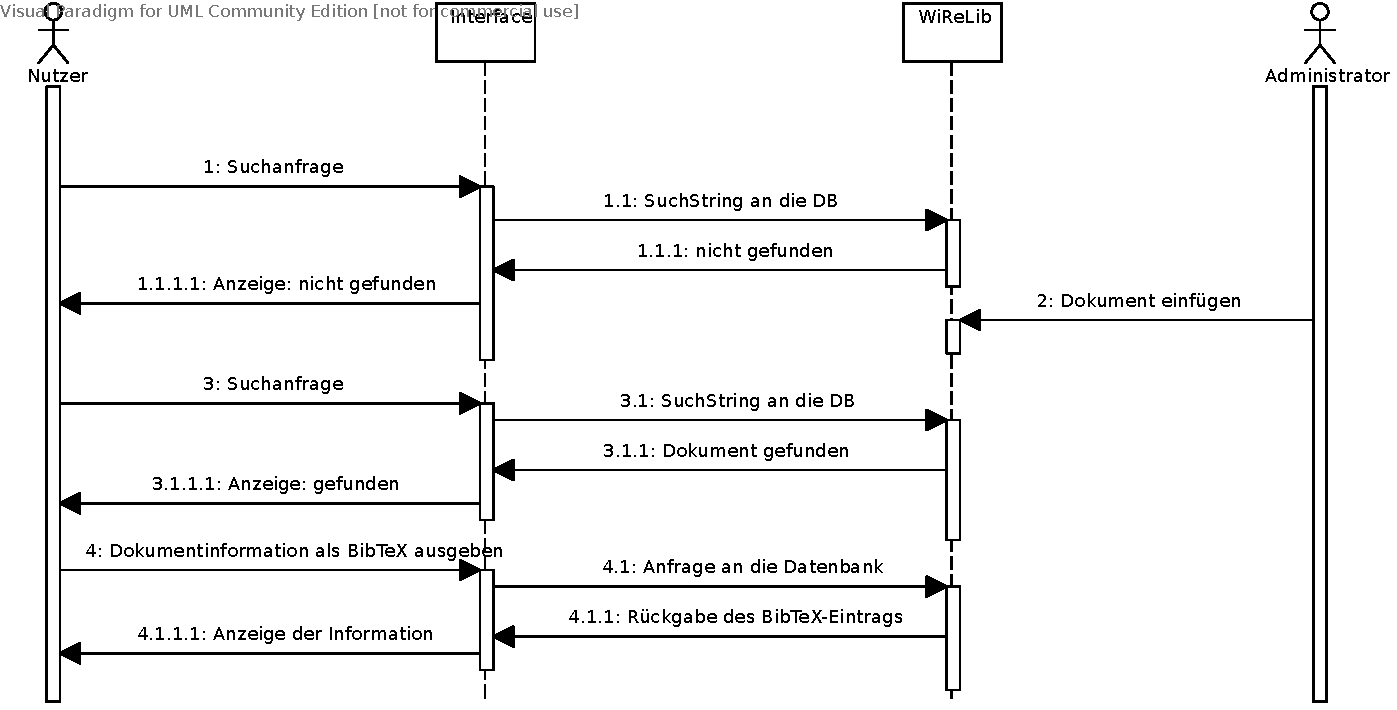
\includegraphics[width=0.8\linewidth]{bilder/Seq-Uebersicht.pdf}
\caption[Übersichtssequenzdiagramm]{Übersichtssequenzdiagramm}
\label{fig:Seqü}
\end{figure}

\subsection{Client}
Über das Web-Interface erhält der als Client fungierende Browser Zugriff auf die Datenbank und kann verschiedene Funktionen nutzen.

\subsection{Server}
Auf dem Server läuft die Anwendung, welche verschiedene Funktionen zum Auslesen und Verwalten der Datenbank bereitstellt. 
Auch stellt der Server die Datenbank bereit und baut eine sichere Verbindung zum Client auf.

\subsection{Datenbank}
In der Datenbank werden die Dokumenente sowie die Nutzerrechte verwaltet.
Auch werden Daten zu den einzelnen Nutzern gespeichert um diese zu identifizieren und im Falle des Ablaufs der Verleihfrist zu benachrichtigen.
               % Kapitel 1
% Kapitel 2 mit den entsprechenden Unterkapiteln
% Die Unterkapitel können auch in separaten Dateien stehen,
% die dann mit dem \include-Befehl eingebunden werden.
%-------------------------------------------------------------------------------
\chapter{Erfüllung der Kriterien}

Nachfolgend wird beschrieben, wie die einzelnen Kriterien des Pflichtenheftes
erfüllt werden und worauf geachtet wird.
\section{Musskriterien}

Die folgenden Kriterien sind unabdingbar und werden durch das Produkt erfüllt:
\begin{description}
  \item[/M10/] Es muss eine gut funktionierende Suchfunktion vorhanden sein.
  \item[/M20/] Den Benutzern werden verschiedene Rollen zugewiesen.
  \item[/M21/] Gäste können Bücher suchen und sich Informationen zu diesen
	anzeigen lassen.
  \item[/M22/] Normale Nutzer können auf alle Funktionen, die für den
	allgemeinen Gebrauch nötig sind, zugreifen. So zum Beispiel
	das Entleihen von Dokumenten oder die Einsicht in ihre derzeitig
	ausgeliehen Dokumente.
  \item[/M23/] Die Benutzerverwaltung wird durch die Rolle User-Admin realisiert.
  \item[/M24/] Der Bibliothekar besitzt Verwaltungsrechte für Dokumente.
  \item[/M25/] Der Administrator besitzt Vollzugriff auf das System.
  \item[/M30/] Es ist für \gls{glos:ext} möglich, sich ein Dokument auszuleihen,
	indem ihnen ein registrierter Nutzer dieses überträgt.
  \item[/M40/] Jedes Dokument besitzt verschiedene Eigenschaften, wie eine
	Kategorie, Autoren und weitere. Auch kann eine Ausleih-Historie zu jedem
	Dokument abgefragt werden.
  \item[/M50/] Das Layout ist an das \gls{glos:copdes} der Technischen
	Universität Braunschweig angepasst und ist klar strukturiert.
  \item[/M60/] Für die Zeichencodierung wird UTF-8, welches eine Form von
	\gls{glos:unicode} ist, verwendet.
	Ein Import von \gls{glos:BibTeX} Dateien ist möglich, sowie ein Export in
	\gls{glos:BibTeX}, als Backup, und eine adt-Datei für \gls{glos:Allegro}.
  \item[/M70/] Für den sicheren Datentransfer wird \gls{glos:ssl}/\gls{glos:https} verwendet.
\end{description}

\section{Wunschkriterien}
Die Erfüllung folgender Kriterien für das abzugebende Produkt wird angestrebt:
\begin{description}
  \item[/W10/] Die einzelnen Rechte von Rollen können flexibel zu jeder Zeit
	von der Verwaltung oder dem Administrator geändert werden. Dieses
	Kriterium wird erfüllt.
  \item[/W20/] Ein Filter in der Suche nach dem Vorbild des \gls{glos:thmefi}s.
  \item[/W30/] Verschicken von Erinnerungsmails, sobald die Ausleihfrist
	abgelaufen ist.
  \item[/W40/] Eine Authentifizierung über \gls{LDAP} wird nicht realisiert werden.
\end{description}

\section{Abgrenzungskriterien}
Folgende Funktionalitäten werden nicht durch das Produkt, sondern wie folgt
beschrieben anderweitig erfüllt:
\begin{description}
\item[/A10/] Es findet kein direkter Datentransfer mit der \gls{UB} statt.
	Dies wird über den Export einer adt-Datei, welche für \gls{glos:Allegro}
	lesbar ist, realisiert.
  \item[/A20/] Das System wird nicht darauf ausgelegt, mehr als 100 Benutzer
	oder mehr als 5000 Dokumente zu beinhalten.
  \item[/A30/] Es wird keine Möglichkeit geben, sich das Layout in einer anderen
	Sprache, außer Deutsch, anzeigen zu lassen.
  \item[/A40/] Bei Importfehlern wird keine dynamische Fehlerbehebung 
	durchgeführt. Es wird ein Zeichen gesetzt, dass der Datensatz fehlerhaft
	ist, und muss dann manuell behoben werden.
  \item[/A50/] Es wird kein spezielles Layout für mobile Endgeräte erstellt.
\end{description}
      % Kapitel 2
% Kapitel 3 mit den entsprechenden Unterkapiteln
% Die Unterkapitel können auch in separaten Dateien stehen,
% die dann mit dem \include-Befehl eingebunden werden.
%-------------------------------------------------------------------------------
\chapter{Implementierungsentwurf}
%Dieser Abschnitt hat die Aufgabe, alle verwendeten Klassen und Bibliotheken zu
%dokumentieren. Dabei wird jede Komponente aus dem Grobentwurf gesondert
%betrachtet. F\"ur Entwurfsentscheidungen, die mehr als eine Komponente betreffen,
%wird mit Verweisen zwischen den Dokumentationen der Komponente gearbeitet.  Es
%sind dabei so viele Unterabschnitte einzuf\"ugen, wie Komponenten vorhanden sind.


\section{Gesamtsystem}
%F\"ugen Sie hier bitte das Komponentendiagramm aus dem Grobentwurf ein und
%erl\"autern Sie kurz die Funktionen der Komponenten.
\begin{figure}[!htb]
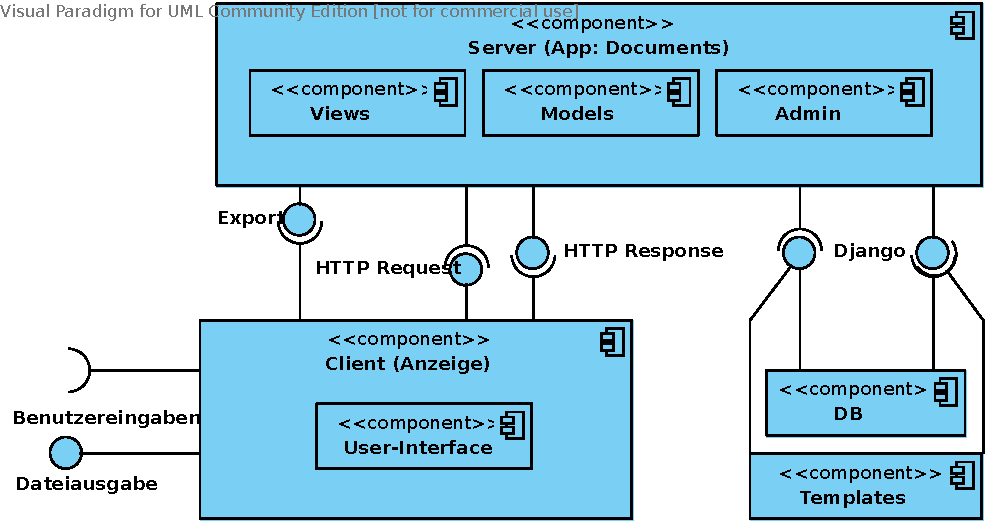
\includegraphics[width=0.8\linewidth]{bilder/Komponentendiagramm.pdf}
\caption{Komponentendiagramm}
\label{fig:KompDiagramm}
\end{figure}

Die Komponente Clent fungiert als Schnittstelle zwischen Benutzer und der 
Applikation Documents. Sie nimmt Eingaben des Benutzers entgegen und bereitet 
HttpResponses des Servers auf.

Die Komponente Views prozessiert HttpRequests des Clients, leitet Aufrufe an die
jeweiligen Templates weiter und füllt diese mit geforderten Informationen.

Die Komponente Models bildet die Struktur der DB ab.

Die Komponente Admin stellt die gesamten Admin-Funktionen zur Verfügung, also 
Funktionen, welche nicht von normalen Benutzern durchgeführt werden sollen.

Die Komponente DB stellt die Datenbank der gesamten Applikation dar.
Sie liefert gewünschte Informationen, z.B. über Dokumente, Benutzer, deren 
ausgeliehenen Bücher etc.

Die Komponente Templates stellt die HTML-Seiten dar, welche durch andere 
Komponenten(Views,Admin...) mit Informationen befüllt    



\section{Implementierung von Komponente
         1: Client:}

%Beschreiben Sie hier bitte die Implementierung der Komponente. Erl\"autern Sie
%bitte dabei, welche Entwurfsmuster und Bibliotheken Sie verwenden. Die
%Implementierung wird dabei durch Klassendiagramme dokumentiert.

Der Client dient als Schnittstelle des Benutzers mit dem eigentlichen Programm
auf dem Server. Mittels eines Browsers der von uns nicht festgelegt wird, werden
die Webseitencodes, die der Server an den Clienten auf dessen Anfragen sendet,
in die für den Benutzer verständliche Form einer Webseite gebracht.

\subsection{Paketdiagramm}
\begin{figure}[!htb]
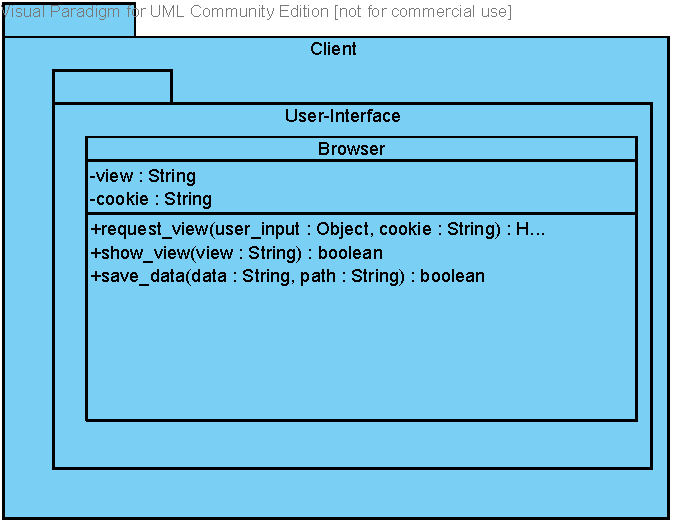
\includegraphics[width=0.8\linewidth]{bilder/Paketdiagramm_client.pdf}
\caption{Paketdiagramm Client}
\label{fig:PDclient}
\end{figure}
\subsection{Erl\"auterung}

Da als Client mehrere verschieden Browser in Frage kommen, können die genauen
Funktionen dieser Komponente hier nicht beschrieben werden. Die für uns
wichtigen Funktionen sind die Möglichkeit eine Anfrage an unseren Server zu
stellen, einen Webseitencode darstellen zu können und eine Datei lokal zu
speichern. Dabei funktioniert die Kommunikation mit dem Server über
Http-Requests und Http-Responses. Für die Korrektheit der Ergebnisse mancher
Anfragen wird der lokale Cookie benötigt und deswegen mitgesendet. 
Auf eine Anfrage per HttpRequest kann der Browser entweder einen Webseitencode 
oder eine Datei als Http-Response erhalten. Je nachdem was er erhält, ruft er 
die passende Funktion auf. 

%Die verwendeten Attribute, Aufgaben und Kommunikationspartner sind f\"ur jede
%Klasse kurz zu erl\"autern. Die ankommenden Nachrichten beziehen sich dabei auf
%die Sequenzdiagramme der Feinanalyse im Grobentwurf und stellen meist
%aufzurufende Methoden der Klasse dar.  Reine get- / set-Methoden oder
%Bibliotheksfunktionen brauchen nicht aufgef\"uhrt zu werden.

\section{Implementierung von Komponente
         2: View:}

%Beschreiben Sie hier bitte die Implementierung der Komponente. Erl\"autern Sie
%bitte dabei, welche Entwurfsmuster und Bibliotheken Sie verwenden. Die
%Implementierung wird dabei durch Klassendiagramme dokumentiert.

Die Views sind einer der essentiellen Bestandteile des Django-Frameworks. Sie
bestimmen die Art und Weise wie Templates aufgerufen werden, welche
Informationen die Templates bekommen und wie die Daten aus den Templates
verarbeitet werden. Sie sind die Schnittstelle zwischen den Templates und dem
Rest des Programms.

\subsection{Paketdiagramm}
\begin{figure}[!htb]
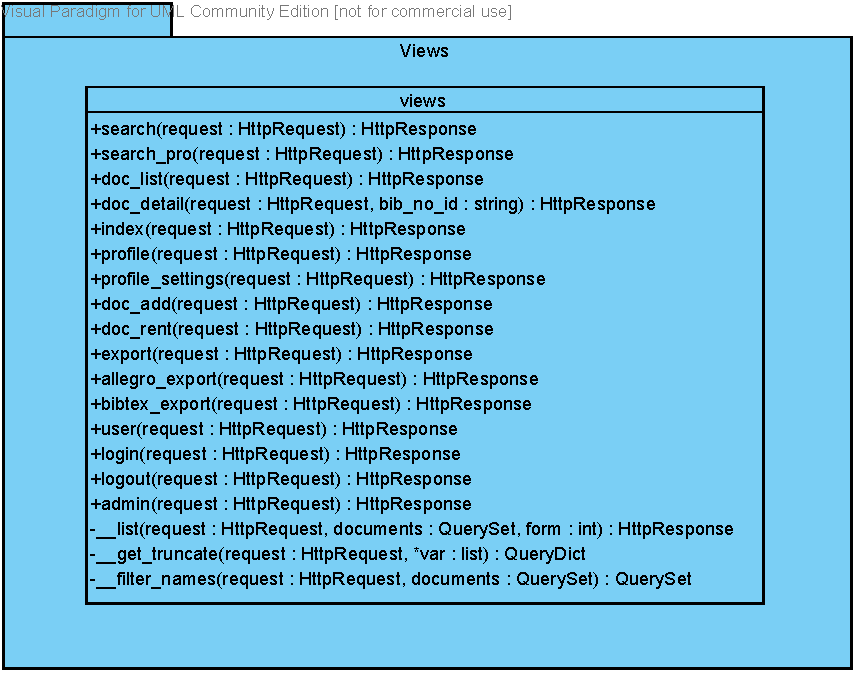
\includegraphics[width=0.8\linewidth]{bilder/Paketdiagramm_views.pdf}
\caption{Paketdiagramm Views}
\label{fig:PDviews}
\end{figure}
\subsection{Erl\"auterung}
Die Komponente View besteht aus einem einzigen Paket, welches für jede
beachbsichtigte Art des Aufrufs eines Templates eine Funktion zur Verfügung
stellt. Dabei erhalten die Funktionen über einen Http-Request Informationen die
in der Funktion verarbeitet werden und geben einen Http-Response zurück, welche
den fertigen Webseitencode enthält. Da die Funktion doc\_detail benötigt
teilweise indirekt von anderen Funktionen der Komponente view aufgerufen wird
benötigt sie noch den zusätzlichen Parameter der ihr mitteilt, welches Dokument
dargestellt werden soll.


\section{Implementierung von Komponente
         3: Models:}

%Beschreiben Sie hier bitte die Implementierung der Komponente. Erl\"autern Sie
%bitte dabei, welche Entwurfsmuster und Bibliotheken Sie verwenden. Die
%Implementierung wird dabei durch Klassendiagramme dokumentiert.

Die Komponente Models stellt die Struktur der Datenbank dar. Das
Django-Framework nimmt diese Struktur und setzt sie selbstständig in eine SQLite Datenbank
um. Jede Klasse dieser Komponente ist das Muster für eine Tabelle in der
Datenbank.

\subsection{Paketdiagramm}
\begin{figure}[!htb]
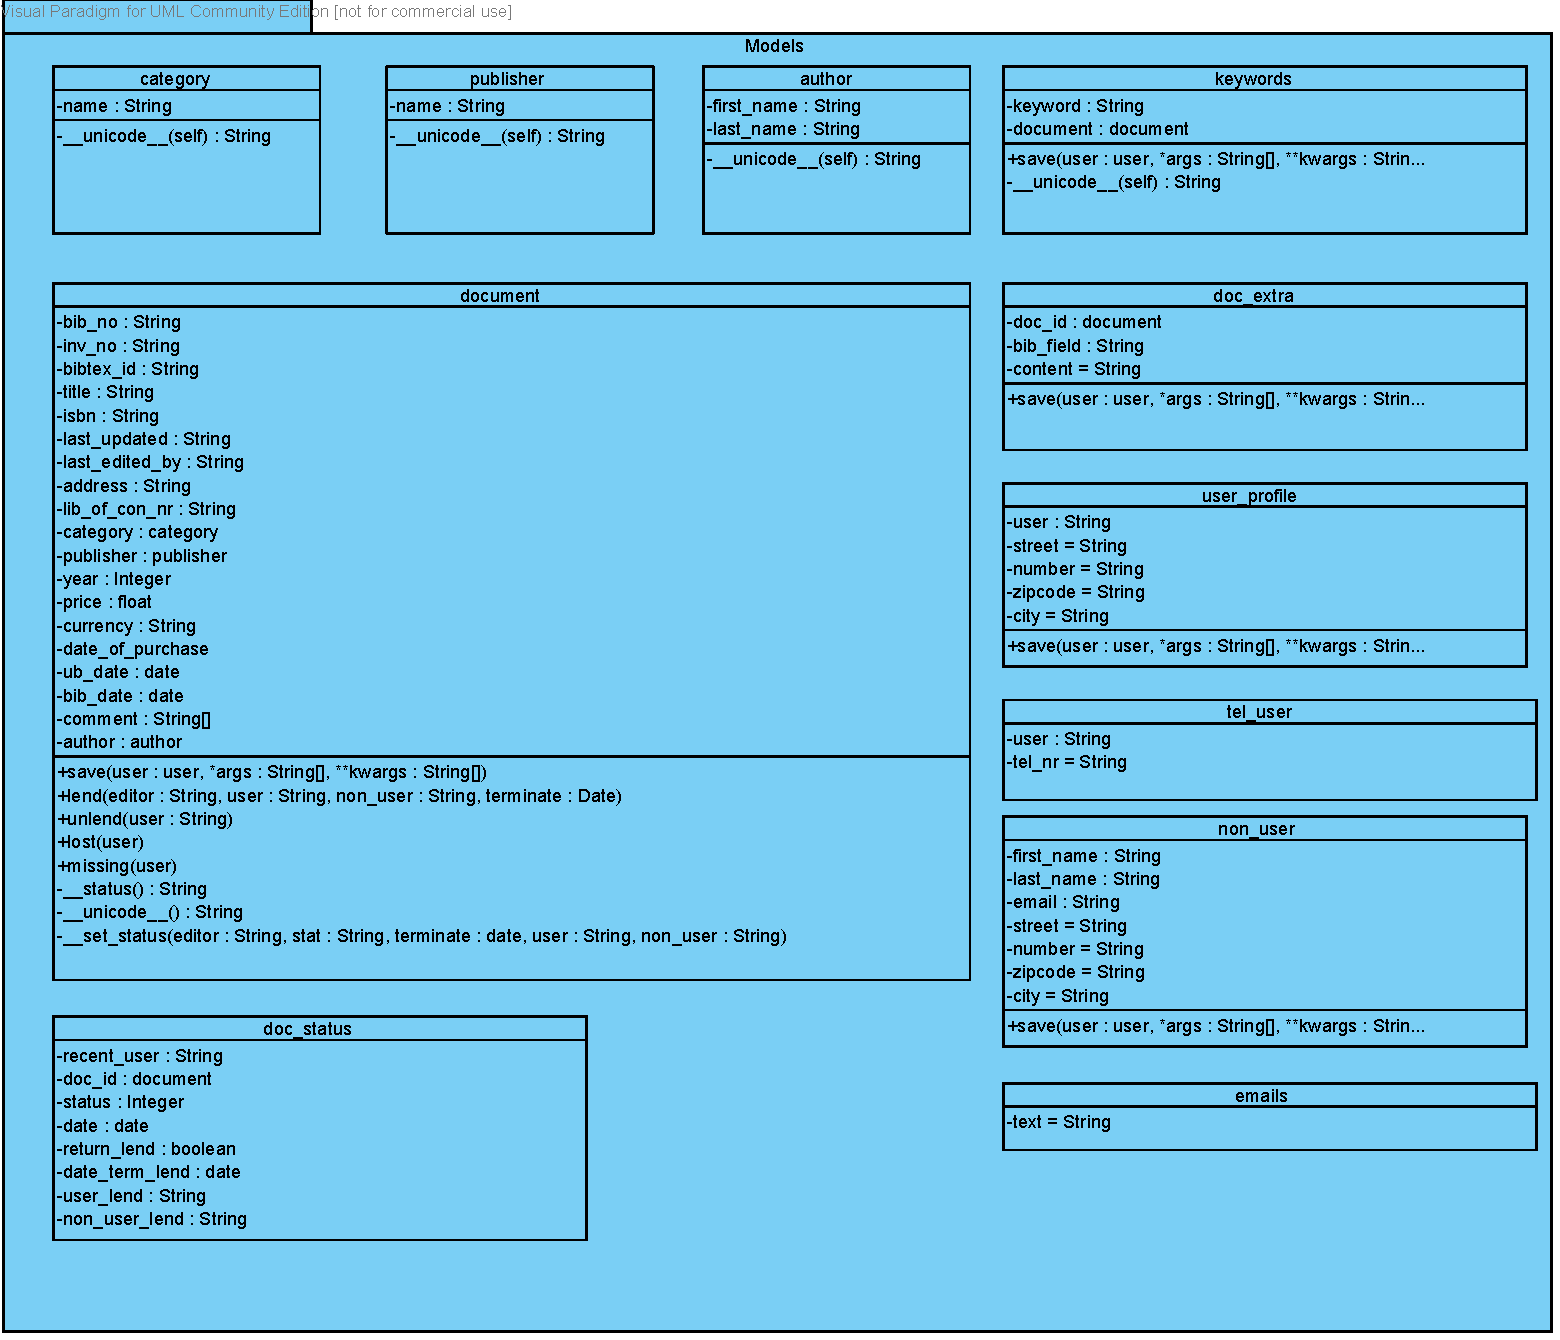
\includegraphics[width=0.8\linewidth]{bilder/Paketdiagramm_models.pdf}
\caption{Paketdiagramm Models}
\label{fig:PDmodels}
\end{figure}
\subsection{Erl\"auterung}
Jede Klasse stellt eine Tabelle in der Datenbank dar und jedes Attribut eine
Spalte dieser Tabelle. Wenn ein Attribut den Typ einer anderen Klasse aus den
Models besitzt stellt dies eine Beziehung in der späteren Datenbank dar.
Mehrere Klassen haben die unicode-Funktion. Diese Funktion definiert wie eine
Tabelle bzw. eine Zeile dieser Tabelle als String dargestellt werden soll.
Mehrere Klassen haben die save-Funktion, welche gerade durchgeführte Änderungen
unter Angabe des Editors sofort speichert. Die Klasse \"documents\" hat außerdem
die Funktionen lost, missing, unlend und lend welche den Status des jeweiligen
Dokumentes ändern können.

\section{Implementierung von Komponente
         4: Admin:}

%Beschreiben Sie hier bitte die Implementierung der Komponente. Erl\"autern Sie
%bitte dabei, welche Entwurfsmuster und Bibliotheken Sie verwenden. Die
%Implementierung wird dabei durch Klassendiagramme dokumentiert.

Die Komponente Admin stellt die Funktionen zur Veränderung von Daten Verfügung, die nicht von
normalen Benutzern durchgeführt werden sollen.

\subsection{Paketdiagramm}
\begin{figure}[!htb]
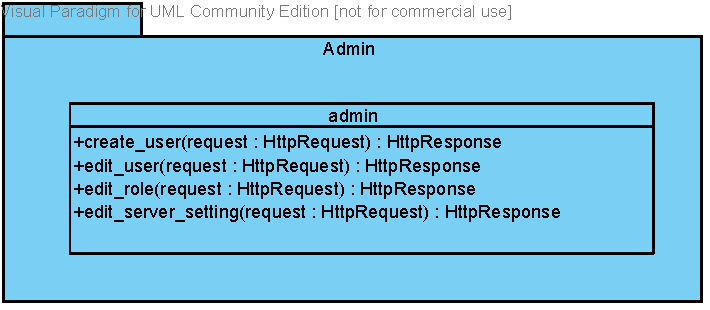
\includegraphics[width=0.8\linewidth]{bilder/Paketdiagramm_admin.pdf}
\caption{Paketdiagramm Admin}
\label{fig:PDadmin}
\end{figure}
\subsection{Erl\"auterung}
Die Eingabe der Daten für die Adminofunktionen funktioniert auch hier über
einen Http-Request. Die Http-Response besteht hier allerdings nur aus einer
Nachricht, dass die Änderung funktioniert hat und eventuell der Ansicht der
geänderten Daten. Es ist mit diesen Funktionen möglich in der Datenbank neue
User zu erstellen und zu ändern, die verfügbaren Rollen zu bearbeiten und die
gerellen Einstellungen des Servers zu ändern. 

\section{Implementierung von Komponente
         5: DB und Template:}

%Beschreiben Sie hier bitte die Implementierung der Komponente. Erl\"autern Sie
%bitte dabei, welche Entwurfsmuster und Bibliotheken Sie verwenden. Die
%Implementierung wird dabei durch Klassendiagramme dokumentiert.

Die Datenbank ist eine SQLite Datenbank. Dabei übernimmt allerdings das
Django-Framework die komplette Kommunikation mithilfe der Komponente Models. 
Die Templates sind eine statische Komponente auf die das Django-Framework
zugreift sobald sie von der Komponente View benötigt werden. 

\subsection{Paketdiagramm}
Die Paketdiagramme wurden weggelassen. Siehe dazu den Punkt Erläuterung.

\subsection{Erl\"auterung}
Die Datenbank ist eine SQLite-Datenbank. Ein Paketdiagramm für das komplette
SQLite würde die Maße dieses Dokumentes sprengen und wird deswegen weggelassen.
Auf ein Paketdiagramm für die Komponente Templates wird verzichtet, da diese
keinerlei Funktionen besitzt sondern nur von anderen Komponenten mit Daten
gefüllt und weitergeleitet wird. Diese Kommunikation wird von Django-Framework
durchgeführt für das ein Paketdiagram ebenfalls die Maße dieses Dokumentes
sprengen würde.
  % Kapitel 3
% Kapitel 4 mit den entsprechenden Unterkapiteln
% Die Unterkapitel können auch in separaten Dateien stehen,
% die dann mit dem \include-Befehl eingebunden werden.
%-------------------------------------------------------------------------------
\chapter{Datenmodell}
Falls in der Anwendung bestimmte Daten dauerhaft gespeichert werden, so sind
die entsprechenden Entities und Beziehungen hier darzustellen und zu erl\"autern.
Dies ist insbesondere relevant, falls der Einsatz einer (relationalen)
Datenbank geplant ist.

\section{Diagramm}


\begin{figure}[!htb]
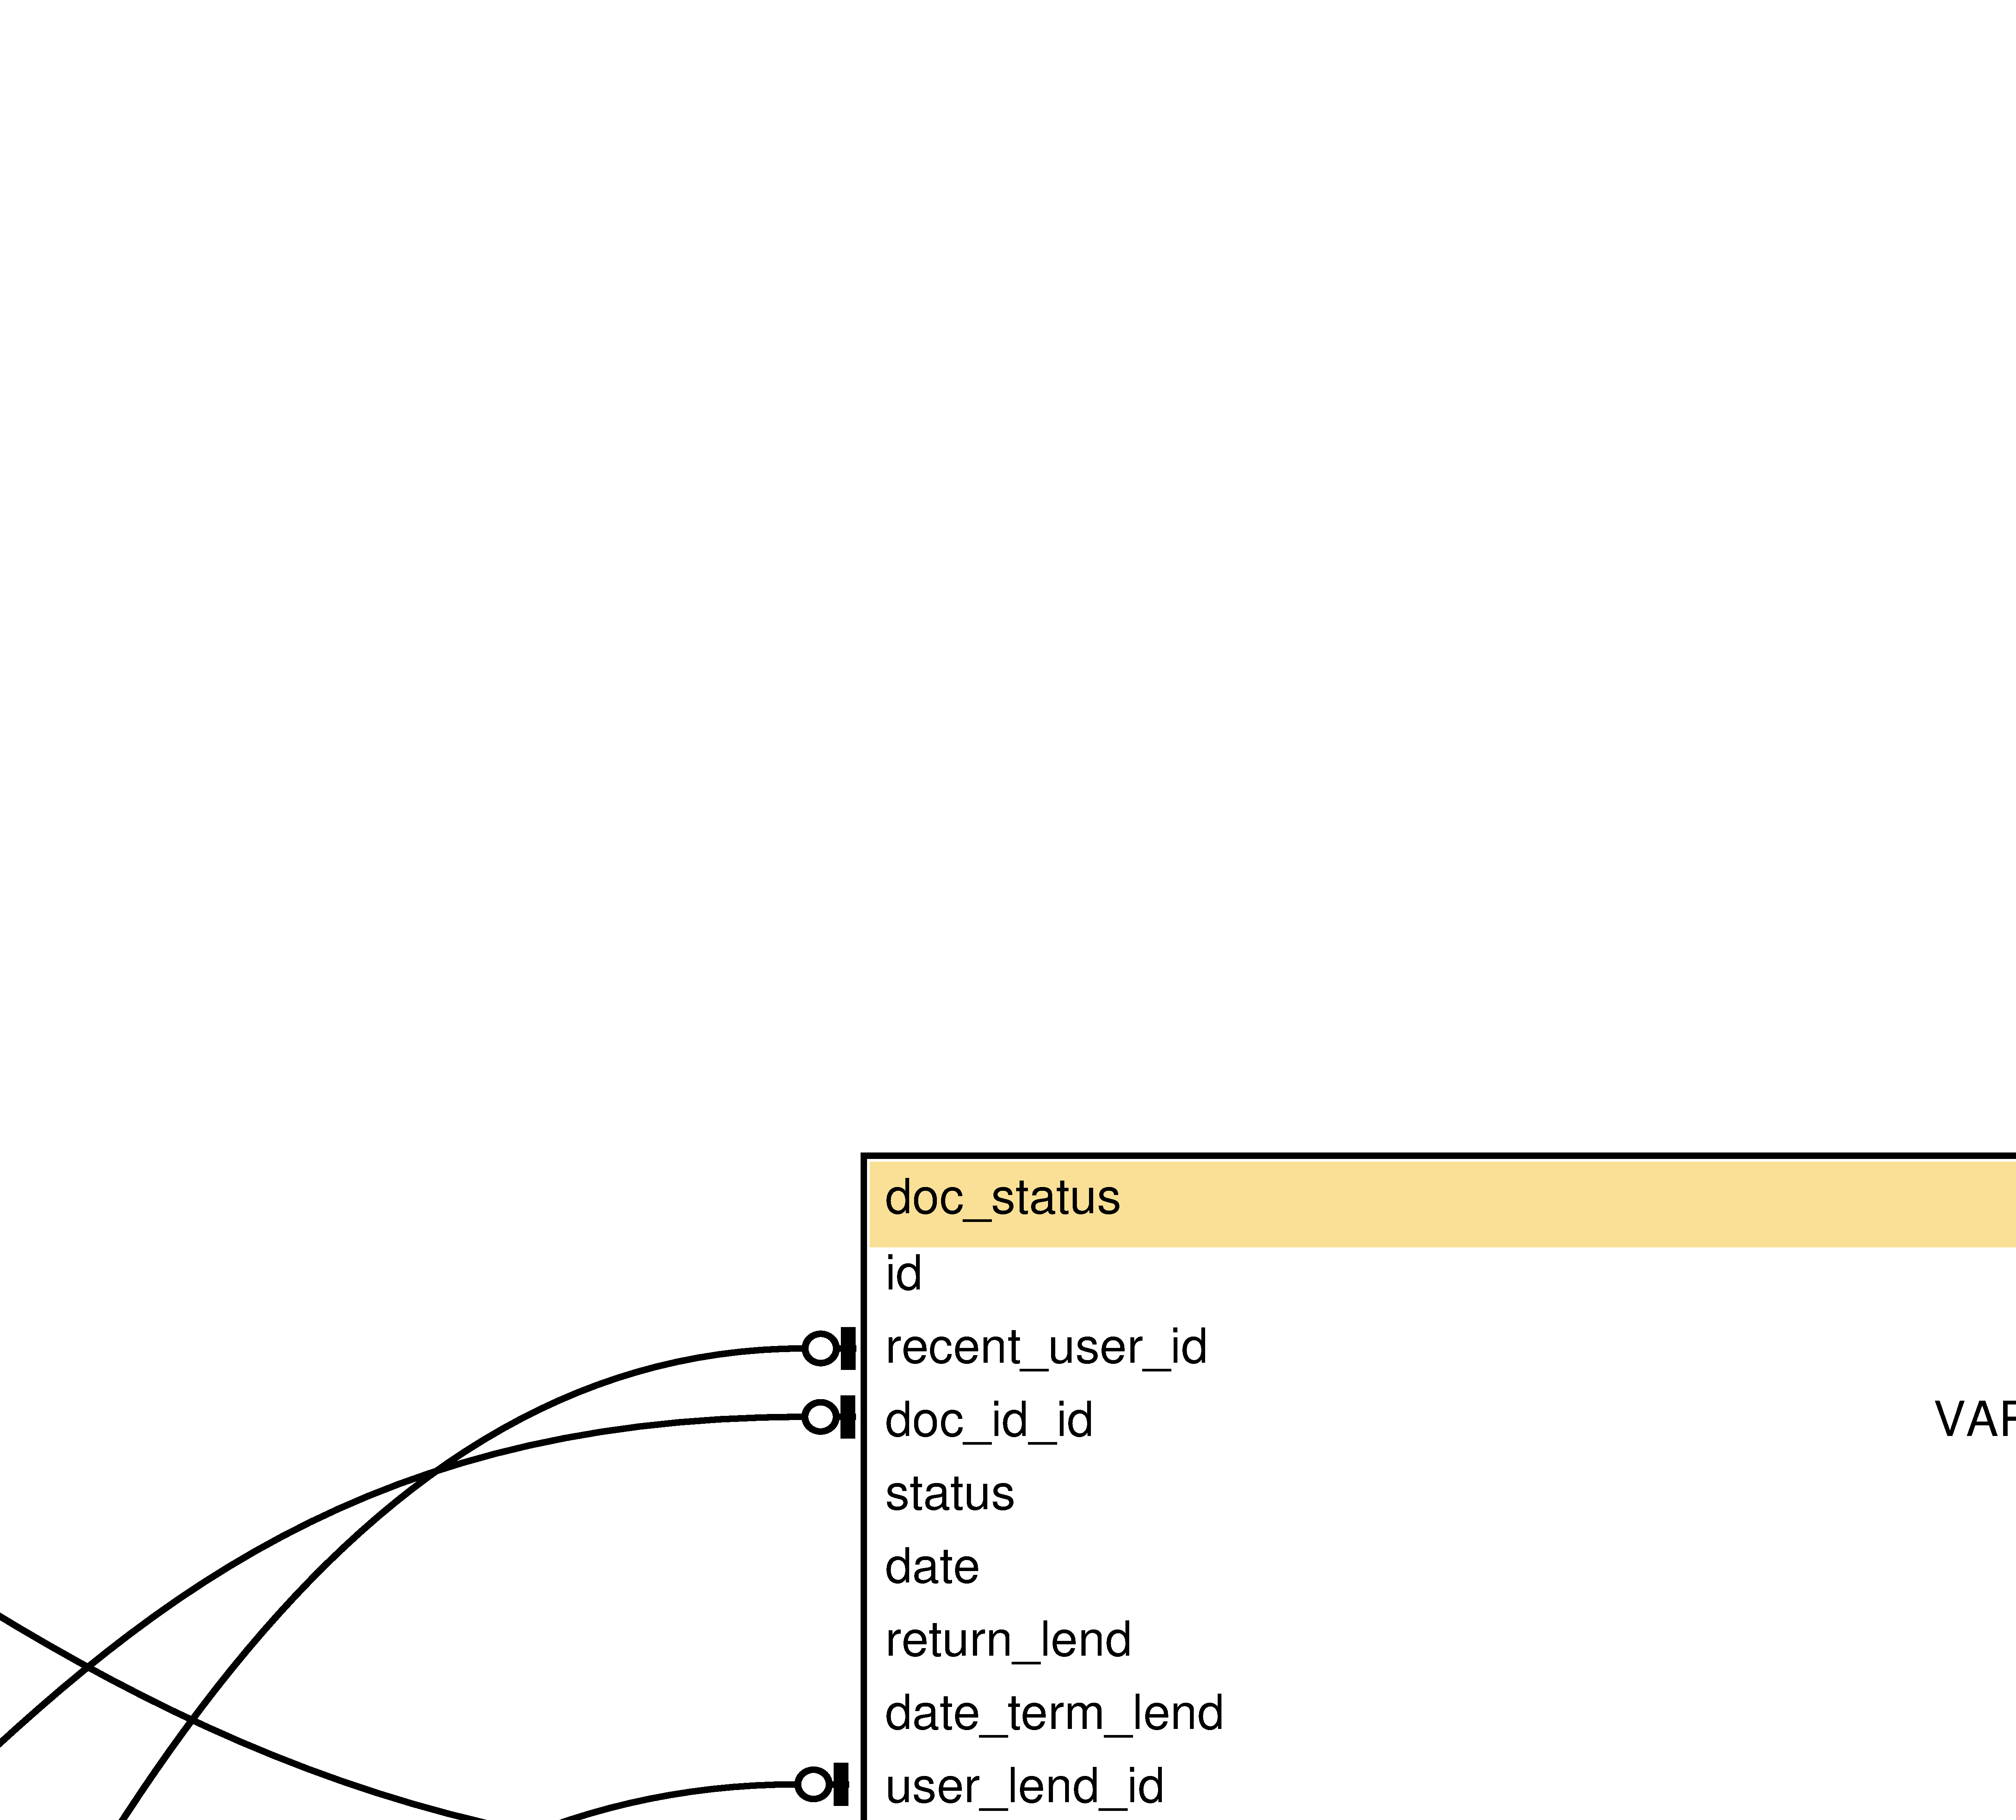
\includegraphics[width=0.8\linewidth]{bilder/database-wirelib.pdf}
\caption{Datenbankmodell}
\label{fig:DBDiagramm}
\end{figure}

Das Diagramm gibt eine grobe Übersicht über die Struktur der zugrundeliegenden
relationalen Datenbank. Im Folgenden werden die beiden wichtigsten
Teilstrukturen der Datenbank für bessere Übersicht dargestellt.


\begin{figure}[!htb]
\includegraphics[width=1\linewidth]{bilder/database-wirelib_cluster-doc.pdf}
\caption{Datenbankmodell: Bibliothek}
\label{fig:DB_docDiagramm}
\end{figure}

Dieses Diagramm gibt eine Übersicht über alle Tabellen der Datenbank, die im
Zusammenhang mit der Bibliothek stehen. Die wichtigste Tabelle ist document, in
der die vorhandenen Dokumente eingetragen werden. In der Tabelle doc\_status
werden alle Statusänderungen eines Dokumentes festgehalten, einschließlich der
Ausleihe eines Dokumentes. Die Tabelle doc\_extra speichert zusätzliche Inhalte
eines Dokumentes, die aufgrund seltenen Gebrauchs nicht lohnen, in document
direkt aufgenommen zu werden. In der Tabelle emails werden die E-Mail-Templates
gespeichert, die verschickt werden, wenn die Ausleihfrist eines Dokumentes
abläuft oder in ähnlichen Fällen. Die Tabellen auth\_user und non\_user sind
in der Teilstruktur Benutzer und hier nur als Referenz gedacht zur besseren
Übersicht. Die verbleibenden Tabellen speichern trivialerweise den
beschriebenen Inhalt.


\begin{figure}[!htb]

\includegraphics[width=1\linewidth]{bilder/database-wirelib_cluster-user.pdf}
\caption{Datenbankmodell: Benutzer}
\label{fig:DB_UserDiagramm}
\end{figure}

Dieses Diagramm gibt eine Übersicht über alle Tabellen der Datenbank, die im
Zusammenhang mit Benutzerverwaltung stehen. Alle Tabellen, die in diesem Modell
mit dem Präfix \emph{auth\_} beginnen, sind von Django generiert und werden für
eine erleichterte Handhabung von Benutzern und Rechtevergabe genutzt. Tabellen
mit dem Präfix \emph{django\_} werden ebenfalls von Django generiert und dienen
dem Admin-Interface von Django und dem Session-Managment von eingeloggten
Benutzern. Die Tabelle non\_user ist für Nutzer gedacht, die nicht am Institut
für Wissenschaftliches Rechnen arbeiten und trotzdem ein Dokument ausleihen
wollen. Sie haben so keine Möglichkeit, sich auf der Webseite einzuloggen,
können aber trotzdem Dokumente ausleihen. Die Tabellen tel\_user und
tel\_non\_user werden benötigt, um Telefonnumern zu Benutzern zu speichern.
user\_profile ist zur Erweiterung der Django-Tabelle auth\_user, um auch
Adressen speichern zu können.

% Eigenes Klassendiagramm einsetzen
\section{Erl\"auterung}

\begin{longtable}{|p{5cm}||m{5cm}|c|}
  \hline
  Entit\"at & \multicolumn{2}{c|}{Beziehungen} \\
  \hline\hline\hline
  
  author  & Name der Beziehung &  Kardinalit\"at\\
  \hline\hline
  document\_authors & hat geschrieben & 1,n \\
  \hline\hline\hline
  
  document\_authors & Name der Beziehung & Kardinalität\\
  \hline\hline
  author & wurde geschrieben von & 1\\
  \hline
  document & hat geschrieben & 1\\
  \hline\hline\hline
  
  document: & Name der Beziehung & Kardinalität\\
  \hline\hline
  document\_authors & wurde geschrieben von & 1,n\\
  \hline
  category & gehört zur Kategorie & 1\\
  \hline
  publisher & wurde veröffentlicht von & 1\\
  \hline
  keywords & besitzt die Schlüsselwörter & n\\  
  \hline
  doc\_extra & besitzt die Extrafelder & n\\
  \hline
  doc\_status & hat den Status/verliehen an & n\\
  \hline\hline\hline
  
  keywords:  & Name der Beziehung &  Kardinalit\"at\\
  \hline\hline
  document & gehört zum Dokument & 1 \\
  \hline\hline\hline
  
  publisher:  & Name der Beziehung &  Kardinalit\"at\\
  \hline\hline
  document & hat veröffentlicht & 1,n \\
  \hline\hline\hline
  
  category:  & Name der Beziehung &  Kardinalit\"at\\
  \hline\hline
  document & enthält & n \\
  \hline\hline\hline
  
  doc\_extra:  & Name der Beziehung &  Kardinalit\"at\\
  \hline\hline
  document & gehört zu & 1 \\
  \hline
  \pagebreak
  \hline\hline
  
  doc\_status: & Name der Beziehung & Kardinalität\\
  \hline\hline
  document & gehört zum Dokument & 1\\
  \hline
  auth\_user & wurde geändert von & 1\\
  \hline
  auth\_user & wurde ausgeliehen von & 0,1\\
  \hline
  non\_user & wurde weitergegeben an & 0,1\\
  \hline\hline\hline
  
  non\_user: & Name der Beziehung & Kardinalität\\
  \hline\hline
  doc\_status & entlieh & 1,n\\
  \hline
  tel\_non\_user & hat die Telefonnummern & 1,n\\
  \hline\hline\hline
  
  tel\_non\_user:  & Name der Beziehung &  Kardinalit\"at\\
  \hline\hline
  non\_user & gehört zu & 1 \\
  \hline\hline\hline
  
  auth\_user: & Name der Beziehung & Kardinalität\\
  \hline\hline
  user\_profile & wohnt & 1\\
  \hline
  tel\_user & hat die Telefonnumern & 1,n\\
  \hline
  auth\_user\_user\_permissions & hat die Rechte & n\\
  \hline
  doc\_status & änderte den Status & n\\  
  \hline
  doc\_status & leiht/bürgt gerade für & n\\
  \hline
  django\_admin\_log & aktualisiert & n\\
  \hline
  auth\_message & bekam & n\\
  \hline\hline\hline
  
  tel\_user:  & Name der Beziehung &  Kardinalit\"at\\
  \hline\hline
  auth\_user & gehört zu & 1 \\
  \hline\hline\hline 
  
  auth\_message: & Name der Beziehung &  Kardinalit\"at\\
  \hline\hline
  auth\_user & gesendet an & 1 \\
  \hline\hline\hline 
  
  user\_profile:  & Name der Beziehung &  Kardinalit\"at\\
  \hline\hline
  auth\_user & Anschrift von & 1 \\
  \hline\hline\hline
  
  auth\_user\_groups:  & Name der Beziehung &  Kardinalit\"at\\
  \hline\hline
  auth\_user & der User & 1 \\
  \hline
  auth\_group & gehört zur Gruppe & 1 \\
  \hline\hline\hline
  
  auth\_group: & Name der Beziehung &  Kardinalit\"at\\
  \hline\hline
  auth\_user\_groups & besitzt die Mitglieder & n \\
  \hline
  auth\_group\_permissions & hat die Rechte & n \\
  \hline\hline\hline 

  auth\_group\_permissions: & Name der Beziehung &  Kardinalit\"at\\
  \hline\hline
  auth\_group & die Gruppe & 1 \\
  \hline
  auth\_permission & hat das Recht & 1 \\
  \hline
  \pagebreak
  \hline\hline 
  
  auth\_user\_user\_permissions:  & Name der Beziehung &  Kardinalit\"at\\
  \hline\hline
  auth\_user & der User & 1 \\
  \hline
  auth\_permission & hat das Recht & 1 \\
  \hline\hline\hline 
  
  auth\_permission:  & Name der Beziehung &  Kardinalit\"at\\
  \hline\hline
  auth\_user\_user\_permissions & der User hat  & n \\
  \hline
  auth\_group\_permissions & die Gruppe hat & n \\
  \hline
  django\_content\_type & referenziert & 1 \\
  \hline\hline\hline
  
  django\_admin\_log:  & Name der Beziehung &  Kardinalit\"at\\
  \hline\hline
  auth\_user & getätigt von  & 1 \\
  \hline
  django\_content\_type & referenziert & 1 \\
  \hline\hline\hline
  
  django\_content\_type:  & Name der Beziehung &  Kardinalit\"at\\
  \hline\hline
  auth\_permission & stellt Referenz  & n \\
  \hline
  django\_admin\_log & ändert & n \\
  \hline
\end{longtable}
              % Kapitel 4
% Kapitel 5
%-------------------------------------------------------------------------------
\chapter{Serverkonfiguration}
%Sollte ein Server (z.B. Tomcat) f\"ur die Bearbeitung und Nutzung des Produktes
%erforderlich sein, so ist hier dessen Konfiguration zu beschreiben. Dies
%geschieht durch explizite Nennung aller Konfigurationsdateien und notwendiger
%Eintr\"age.
Im folgenden wird eine vollständige Installationsbeschreibung am Beispiel eines
\Gls{glos:ubuntu} Servers mit \Gls{glos:lighttpd} vorgestellt. Diese
Beschreibung berücksichtigt einige Anforderungen für ein Produktivsystem nicht
und ist für ein solches Setup nur als Hilfsreferenz verwendbar. 

Das im folgenden beschriebene Setup weicht in Bezug auf das Datenbanksystem von
dem Pflichtenheft ab, in dem die Verwendung einer \Gls{glos:sqlite}-Datenbank
angesetzt wurde. Dieser Punkt des Pflichtenheftes kann ohne Probleme bei Bedarf
verwendet werden, ist aber aufgrund von Einschränkungen von \Gls{glos:sqlite}
für ein Produktivsystem nicht zu empfehlen\footnote{Eine SQLite Datenbank wird
bei Schreibzugriffen vollständig gesperrt und arbeitet durch ihre Persistenz
langsamer als eine MySQL-Datenbank}.

\section{Installation notwendiger Programme}
Um das System über einen Webserver verfügbar machen zu können, muss erst einmal
die nötige Software installiert werden. In dieser Beschreibung wird auf den
schlanken und flexiblen Webserver \Gls{glos:lighttpd} gesetzt, als
Datenbanksystem wird ein \Gls{glos:mysql} Datenbanksystem verwendet.

Zu installierende Pakete:
\begin{itemize}
  \item lighttpd
  \item mysql-server
  \item python-django
  \item git
  \item python-pip
  \item python-mysqldb
\end{itemize}
Die Installation kann mit \zB \lstinline{apt-get install lighttpd} getätigt
werden.

Sobald diese Pakete installiert sind, muss die \Gls{glos:mysql} Datenbank
vorbereitet werden.

\section{MySQL einrichten}
Um die Datenbank einzurichten, wird in dieser Beschreibung auf das in
\Gls{glos:php} geschriebene Programm \Gls{glos:adminer} zurückgegriffen.
Um dies jedoch verwenden zu können, müssen die folgenden zwei Pakete installiert
werden.

\begin{itemize}
  \item php5-cgi
  \item php5-mysql
\end{itemize}

Für \Gls{glos:adminer} muss zuerst \Gls{glos:php} auf dem Webserver verfügbar
gemacht werden. Dazu sind folgende Anpassungen an \Gls{glos:lighttpd}
notwendig:
In der Konfigurationsdatei \emph{/etc/lighttpd/lighttpd.conf} muss zu den
\lstinline{server.modules} das Modul \lstinline{mod_fastcgi} hinzugefügt
werden und am Ende der Konfigurationsdatei folgende Zeilen:

\begin{lstlisting}
fastcgi.server = ( ".php" => (( 
     "bin-path" => "/usr/bin/php-cgi",
     "socket" => "/tmp/php.sock",
     )))
\end{lstlisting}

Nun kann \Gls{glos:adminer} herunter geladen werden und unter \emph{/var/www}
gespeichert werden. Nach einem Neustart von \Gls{glos:lighttpd} mit
\lstinline{service lighttpd restart} kann man über einen Webbrowser Adminer
ansteuern und damit auf die lokale \Gls{glos:mysql}-Datenbank zugreifen. Zuerst
sollten zur Absicherung die leeren Benutzer (über "`Rechte"') von der Datenbank
entfernt werden. Zusätzlich müssen noch die zwei Datensätze, die die leeren
Benutzer betreffen unter "`mysql/db"' gelöscht werden.  Danach wird ein neuer
Benutzer "`wirelib"' mit Rechten auf die Datenbank "`wirelib"' erzeugt. Die
Rechte des Benutzers müssen und sollten nur alle Rechte auf "`Tabelle"' und "`Spalte"'
haben.

Da nun der zukünftige Benutzer auf der Datenbank existiert, muss nur noch die
Datenbank "`wirelib"' erzeugt werden. Die Datenbank heißt "`wirelib"' und
wird auf \lstinline{utf8_unicode_ci} als Zeichensatz eingestellt.

Nach Abschluss dieser Vorbereitungen kann die \emph{adminer.php} gelöscht und
\Gls{glos:php} in \Gls{glos:lighttpd} deaktiviert werden.

\section{Django einrichten}

Um das Produkt unter Django zum laufen zu bringen werden zwei weitere
Python-Pakete benötigt die mittels \Gls{glos:pip} installiert werden können.
Mit 
\begin{lstlisting}
  pip install django-pagination flup
\end{lstlisting}
werden die letzten Abhängigkeiten für das Produkt erfüllt.

\subsection{Django Projekt initieren}

Um das Projekt ein zu richten sind die folgenden Schritte notwendig:
\begin{enumerate}
  \item Mit \lstinline{cd /var/www} in den Webordner wechseln
  \item Mit \lstinline{django-admin startproject wire} das Projekt starten
  \item Mit \lstinline{git clone https://github.com/WiReSEP/WireLib2012.git}
	das Produkt herunterladen
  \item \lstinline{cd /var/www/wire}
  \item \lstinline{ln -s /var/www/WireLib2012/src/wirelib/documents documents}
	fügt das Produkt dem \Gls{glos:django}-Projekt hinzu.
\end{enumerate}

\subsection{Django Projekt einrichten}
Um das Produkt fertig einzurichten müssen im Projekt zwei Dateien editiert
werden, deren Setup im folgenden näher beschrieben wird. Evtl. Anpassungen an
spezielle Bedürfnisse inerhalb einer Django-Projektes müssten wahrscheinlich
hier vorgenommen werden.

\subsubsection{settings.py}
Ein \Gls{glos:django}-Projekt wird über die \emph{settings.py} eingerichtet.
Um das Produkt aber zu verwalten, muss die \emph{settings.py} noch editiert
werden. Den Anfang machen dabei die Zugriffsdaten für die Datenbank, die wie
folgt eingerichtet werden:


\begin{lstlisting}
DATABASES = {
    'default': {
        'ENGINE': 'django.db.backends.mysql',
        'NAME': 'wirelib',
        'USER': 'wirelib', 
        'PASSWORD': 'streng geheim',
        'HOST': 'localhost',
        'PORT': '', #Bei default einfach leer lassen.
    }
}
\end{lstlisting}

Weiter unten in der \emph{settings.py} muss die folgende Middelware aktiv sein:
\begin{lstlisting}
MIDDLEWARE_CLASSES = (
    'django.middleware.common.CommonMiddleware',
    'django.contrib.sessions.middleware.SessionMiddleware',
    'django.middleware.csrf.CsrfViewMiddleware',
    'django.middleware.csrf.CsrfResponseMiddleware',
    'django.contrib.auth.middleware.AuthenticationMiddleware',
    'django.contrib.messages.middleware.MessageMiddleware',
    'pagination.middleware.PaginationMiddleware',
)
\end{lstlisting}

Gefolgt von dem folgenden Templateverzeichnis:
\begin{lstlisting}
TEMPLATE_DIRS = (
    '/var/www/WireLib2012/src/templates',
)
\end{lstlisting}

Damit das Produkt auch verfügbar ist, muss es in der \emph{settings.py} unter
den installierten Apps zu finden sein. Auch zwei Abhängigkeiten müssen zu den
Apps ergänzt werden:
\begin{lstlisting}
INSTALLED_APPS(
    'django.contrib.auth',
    'django.contrib.contenttypes',
    'django.contrib.sessions',
    'django.contrib.sites',
    'django.contrib.messages',
    'django.contrib.staticfiles',
    'django.contrib.admin',
    'pagination',
    'documents',
)
\end{lstlisting}

Zu guter letzt folgen einige Anweisungen für den Template Prozessor:
\begin{lstlisting}
  TEMPLATE_CONTEXT_PROCESSORS = (
    'django.contrib.auth.context_processors.auth',
    'django.core.context_processors.debug',
    'django.core.context_processors.i18n',
    'django.core.context_processors.media',
    'django.core.context_processors.static',
    'django.contrib.messages.context_processors.messages',
    'django.core.context_processors.request'
)
\end{lstlisting}

\subsubsection{urls.py}
Die \emph{urls.py} stellt die Weiche für einkommende Verbindungen dar, alle
Wege auf die Apps und die \emph{views.py} einer jeden App  wird hier
festgelegt.  Für den vollen Funktionsumfang des Produktes wird das
Admin-Backend benötigt. Für dieses Backend muss auch eine entsprechende Weiche
bereit stehen. Weiter wird eine Erweiterung für statische Dateien benötigt, die
nicht von Django interpretiert werden sollen. Zu guter letzt ist natürlich auch
noch ein Eintrag für das Produkt notwendig, der im folgenden Beispiel den
gesammten Root-Ordner mit Außnahme von den Ordnern \emph{static/} und
\emph{admin/}.

\begin{lstlisting}
from django.conf.urls.defaults import patterns, include, url
from django.contrib.staticfiles.urls import staticfiles_urlpatterns

from django.contrib import admin
admin.autodiscover(

urlpatterns = patterns('',
    url(r'^admin/', include(admin.site.urls)),
    url(r'^', include('documents.urls')),
)

urlpatterns += staticfiles_urlpatterns()
\end{lstlisting}

 \subsection{Django Setup abschließen}
 Der Projektordner ist nun bereit für einen Webserver. Was dem Projekt noch
 fehlt, ist die Datenbank, um seine Daten ablegen zu können.

 Die Datenbank wird wie folgt initialisiert:
\begin{lstlisting}
python manage.py syncdb
\end{lstlisting}

\section{Django in Lighttpd verfügbar machen}
In der Datei \emph{/etc/lighttpd/lighttpd.conf} müssen zuerst die nötigen
Module aktiviert werden. Das sind die folgenden:
\begin{lstlisting}
 'mod_fastcgi'
 'mod_rewrite'
\end{lstlisting}

Weiter muss das \emph{document-root} angepasst werden,
\begin{lstlisting}
server.document-root        = "/var/www/wire"
\end{lstlisting}
sowie die folgenden Zeilen der Konfiguration hinzugefügt:
\begin{lstlisting}
fastcgi.server = ( "/wire.fcgi" => (
                "main" => (
                        "socket" => "/var/www/wire/wire.sock",
                        "check-local" => "disable",
                )
        ),
)
alias.url = (
        "/media" => "/usr/lib/python2.7/dist-packages/django/contrib/admin/media/",
        "/static" => "/var/www/static"
)
url.rewrite-once = (
        "^(/wire\.fcgi.*)$" => "$1",
        "^(/media.*)$" => "$1",
        "^(/.*)$" => "/wire.fcgi$1",
)
\end{lstlisting}

 \subsection{Django FCGI-Skript}
Das folgende Skript kann als Grundlage für ein \Gls{cgi}-Start-Skript verwendet
werden. \emph{Wichtig} ist für das Skript allein, dass der Ordner
\lstinline{$PROJECTDIR} dem Benutzer des Webserver (meist \lstinline{www-data})
gehört:

\begin{lstlisting}
chown www-data:www-data /var/www/wire
\end{lstlisting}

Nun das \Gls{cgi}-Skript:
\lstinputlisting{inhalt/django-fcgi}
      % Kapitel 5

%---Hier werden das Glossar und das Abkürzungsverzeichnis gedruckt--------------
\providetranslation{Glossary}{Glossar}
\printglossary[style=altlist,title=Glossar]

\providetranslation{Acronyms}{Akronyme}
\printglossary[type=\acronymtype,style=long]

%------Ende des Dokumentes------------------------------------------------------
\end{document}
